\documentclass[UTF8, 12pt]{ctexart}
% UTF8编码,ctexart现实中文
\usepackage{xcolor}
% 使用颜色
\definecolor{orange}{RGB}{255,127,0}  
\definecolor{violet}{RGB}{192,0,255}  
\definecolor{aqua}{RGB}{0,255,255} 
\usepackage{geometry}
\setcounter{tocdepth}{4}
\setcounter{secnumdepth}{4}
% 设置四级目录与标题
\geometry{papersize={21cm,29.7cm}}
% 默认大小为A4
\geometry{left=3.18cm,right=3.18cm,top=2.54cm,bottom=2.54cm}
% 默认页边距为1英尺与1.25英尺
\usepackage{indentfirst}
\setlength{\parindent}{2.45em}
% 首行缩进2个中文字符
\usepackage{setspace}
\renewcommand{\baselinestretch}{1.5}
% 1.5倍行距
\usepackage{amssymb}
% 因为所以
\usepackage{amsmath}
% 数学公式
\usepackage[colorlinks,linkcolor=black,urlcolor=blue]{hyperref}
% 超链接
\usepackage{tikz}
% 绘图
\author{Didnelpsun}
\title{随机变量及其分布}
\date{}
\begin{document}
\maketitle
\pagestyle{empty}
\thispagestyle{empty}
\tableofcontents
\thispagestyle{empty}
\newpage
\pagestyle{plain}
\setcounter{page}{1}
\section{一维随机变量}

\subsection{随机变量概念}

\textcolor{violet}{\textbf{定义:}}随机变量就是其值会随机而定的变量。设随机试验$E$的样本空间$\Omega={\omega}$,如果对每一个$\omega$都有唯一的实数$X(\omega)$与之对应,并且对任意实数$x$,$\{\omega|X(\omega)\leqslant x,\omega\in\Omega\}$是随机事件,则称定义在$\Omega$上的实值单值函数$X(\omega)$为\textbf{随机变量},记为随机变量$X$。

\subsection{分布函数}

\subsubsection{概念}

\textcolor{violet}{\textbf{定义:}}设$X$为随机变量,$x$为任意实数,称函数$F(x)=P\{X\leqslant x\}$($x\in R$且取遍所有实数)为随机变量$X$的分布函数,或称$X$服从分布$F(x)$,记为$X\sim F(x)$。(随着$x$从$-\infty$到$+\infty$,$X(\omega)$到$\varnothing$到$\Omega$)

\subsubsection{性质}

同样是分布函数的充要条件:

\begin{itemize}
    \item $F(x)$是$x$的单调不减函数,即对任意实数$x_1<x_2$,有$F(x_1)\leqslant F(x_2)$。
    \item $F(x)$是$x$的右连续函数,即对任意$x_0\in R$,有$\lim\limits_{x\to x_0^+}F(x)=F(x_0+0)=F(x_0)$。(左空心右实心)
    \item $F(-\infty)=\lim\limits_{x\to-\infty}F(x)=0$,$F(+\infty)=\lim\limits_{x\to+\infty}F(x)=1$。
\end{itemize}

\subsubsection{应用}

\begin{itemize}
    \item $P\{X\leqslant a\}=F(a)$。
    \item $P\{X<a\}=F(a-0)$。是指分布函数下该点左极限的概率值。
    \item $P(X=a)=F(a)-F(a-0)$。$\because P\{X\leqslant a\}=P\{X<a\cup X=a\}=P\{X<a\}+P\{X=a\}$,$\therefore P\{X=a\}=P\{X\leqslant a\}-P\{X<a\}=F(a)-F(a-0)$。
\end{itemize}

\section{一维离散型随机变量}

\textcolor{violet}{\textbf{定义:}}若随机变量$X$只可能取有限个或可列各值$x_1,x_2,\cdots$,则称$X$为离散型随机变量。

\subsection{分布律}

\textcolor{violet}{\textbf{定义:}}$P\{X=x_i\}=p_i$,$i=1,2,\cdots$为$X$的\textbf{分布列}、\textbf{分布律}或\textbf{概率分布},记为$X\sim p_i$。

概率分布常用表格或矩阵表示:\medskip

\begin{tabular}{c|ccc}
    \hline
    $X$ & $x_1$ & $x_2$ & $\cdots$ \\ \hline
    $P$ & $p_1$ & $p_2$ & $\cdots$ \\
    \hline
\end{tabular}\,或$X\sim\left(\begin{array}{ccc}
    x_1 & x_2 & \cdots \\
    p_1 & p_2 & \cdots
\end{array}\right)$。\medskip

\subsection{性质}

数列$\{p_i\}$是离散型随机变量的概率分布的充要条件是$p_i\geqslant0$($i=1,2,\cdots$)且$\sum\limits_{i=1}^np_i=1$。

设离散型随机变量$X$的概率分布为$P\{X=x_i\}=p_i$,则$X$的分布函数$F(x)=P\{X\leqslant x\}=\sum\limits_{x_i\leqslant x}P\{X=x_i\}$,即离散型随机变量的分布律函数是一个左实右空的阶梯形函数。

$P\{X=x_i\}=P\{X\leqslant x_i\}-P\{X<x_i\}=F(x_i)-F(x_i-0)$,即某点的概率值为该点分布律值减去该点左极限的分布律值。

对实数轴上的任一集合$B$有$P\{X\in B\}=\sum\limits_{x_i\in B}P\{X=x_i\}$,特别地$P\{a<X\leqslant b\}=P\{X\leqslant b\}-P\{X\leqslant a\}=F(b)-F(a)$。

\subsection{应用}

\textbf{例题:}已知随机变量$X$的概率分布为:\medskip

\begin{tabular}{c|ccc}
    \hline
    $X$ & 1 & 2 & 3 \\ \hline
    $P\{X=k\}$ & $\theta^2$ & $2\theta(1-\theta)$ & $(1-\theta)^2$ \\
    \hline
\end{tabular} \medskip

且$P\{X\geqslant2\}=\dfrac{3}{4}$,求未知参数$\theta$与$X$的分布函数$F(x)$。

解:$\because P\{X\geqslant2\}=\dfrac{3}{4}$,$\therefore 2\theta(1-\theta)+(1-\theta)^2=\dfrac{3}{4}$,解得$\theta=\dfrac{1}{2}$,$-\dfrac{1}{2}$舍。

\subsection{分布}

\subsubsection{0-1分布}

\textcolor{violet}{\textbf{定义:}}若$X$的概率分布为$X\sim\left(\begin{array}{cc}
    1 & 0 \\
    p & 1-p
\end{array}\right)$,即$P\{X=1\}=p$,$P\{X=0\}=1-p$,则称$X$服从参数为$p$的0-1分布,记为$X\sim B(1,p)$($0<p<1$)。

0-1分布基于一次伯努利试验,$X$也称为伯努利计数变量。

\subsubsection{二项分布}

\textcolor{violet}{\textbf{定义:}}如果$X$的概率分布为$P\{X=k\}=C_n^kp^k(1-p)^{n-k}$($k=0,1,\cdots,n$,$0<p<1$),则称$X$服从参数为$(n,p)$的\textbf{二项分布},记为$X\sim B(n,p)$。

二项分布基于$n$重伯努利试验。

二项分布的分布律计算,总共进行试验$n$次,已知成功的概率为$p$,若成功了$k$次,则$k$次成功概率为$p^k$,则失败次数为$n-k$,从而$n-k$失败概率为$(1-p)^{n-k}$,因为$n$次试验都是相互独立的,所以将成功的概率与失败的概率乘在一起。又在$n$次中成功$k$次就可以了,进行排列,所以还乘上$C_n^k$。

\subsubsection{泊松分布}

\textcolor{violet}{\textbf{定义:}}如果$X$的概率分布为$P\{X=k\}=\dfrac{\lambda^k}{k!}e^{-\lambda}$($k=0,1,\cdots,n$,$\lambda>0$),则称$X$服从参数为$\lambda$的\textbf{泊松分布},记为$X\sim P(\lambda)$。

泊松分布基于某场合某单位时间内源源不断的质点来流的个数$X=k$,$\lambda$代表质点流动到来的强度。也可以代表稀有事件发生的概率。

\subsubsection{几何分布}

\textcolor{violet}{\textbf{定义:}}如果$X$的概率分布为$P\{X=k\}=(1-p)^{k-1}p$($k=0,1,\cdots,n$,$0<p<1$),则称$X$服从参数为$p$的\textbf{几何分布},记为$X\sim G(p)$。

几何分布与几何无关,代表的是$n$重伯努利试验首次成功就停止试验,试验次数可以为无穷。设$X$表示伯努利试验中事件$A$首次放生所需要的试验次数,则$X\sim G(p)$,其中$p=P(A)$。

从而根据意义,几何分布要求前$k-1$次都失败,从而概率为$(1-p)^{k-1}$,最后一次成功,所以再乘上$p$。

\subsubsection{超几何分布}

\textcolor{violet}{\textbf{定义:}}如果$X$的概率分布为$P\{X=k\}=\dfrac{C_M^kC_{N-M}^{n-k}}{C_N^n}$($\max\{0,n-N+M\}\leqslant k\leqslant\min\{MM,n\}$,$M,N,n$为正整数且$M\leqslant N$,$n\leqslant N$,$k$为整数),则称$X$服从参数为$(n,N,M)$的\textbf{超几何分布},记为$X\sim H(n,N,M)$。

超几何分布考的可能性很小,事件数就是古典概型的一个特例。

如有$N$件产品,其中$M$件正品,从而$N-M$件次品,任取$n$个,则取出$k$件正品的概率就是超几何分布。

\section{一维连续型随机变量}

\textcolor{violet}{\textbf{定义:}}若随机变量$X$的分布函数可以表示为$F(x)=\int_{-\infty}^xf(t)\,\textrm{d}t$($x\in R$且取遍所有实数),其中$f(x)$是非负可积函数,则$X$为\textbf{连续型随机变量}。

\subsection{概率密度}

\textcolor{violet}{\textbf{定义:}}$f(x)$称为$X$的\textbf{概率密度函数},简称\textbf{概率密度},记为$X\sim f(x)$。

\subsection{性质}

改变$f(x)$有限各点的值$f(x)$仍是概率密度(因为单个点没有面积),$f(x)$为某一随机变量$X$的概率密度的充分必要条件:$f(x)\geqslant0$,且$\int_{-\infty}^{+\infty}f(x)\,\textrm{d}x=1$。

若$X$为连续型随机变量,$X\sim f(x)$,则对任意实数$c$有$P\{X=c\}=0$。

对实数轴上的任一集合$B$有$P\{X\in B\}=\int_Bf(x)\,\textrm{d}x$,特别地$P\{a<X<b\}=P\{a\leqslant X<b\}=P\{a<X\leqslant b\}=P\{a\leqslant X\leqslant b\}=\int_a^bf(x)\,\textrm{d}x=F(b)-F(a)$。

\subsection{应用}

\textbf{例题:}已知随机变量$X$的概率密度为$\left\{\begin{array}{ll}
    Ax, & 1<x<2 \\
    B, & 2\leqslant x<3 \\
    0, & \text{其他}
\end{array}\right.$,且$P\{1<X<2\}=P\{2<X<3\}$,求常数$AB$,分布函数$F(x)$以及概率$P\{2<X<4\}$。

解:由于归一性$\int_{-\infty}^{+\infty}f(x)\,\textrm{d}x=1$,$\therefore\int_1^2Ax\,\textrm{d}x+\int_2^2B\,\textrm{d}x=1$。

$\therefore\dfrac{3}{2}A+B=1$。又$P\{1<X<2\}=P\{2<X<3\}$。

$\therefore\int_1^2Ax\,\textrm{d}x=\int_2^3B\,\textrm{d}x$,即$\therefore\int_1^2Ax\,\textrm{d}x=\int_2^2B\,\textrm{d}x=\dfrac{1}{2}$,$A=\dfrac{1}{3}$,$B=\dfrac{1}{2}$。

$f(x)=\left\{\begin{array}{ll}
    \dfrac{1}{3}x, & 1<x<2 \medskip \\
    \dfrac{1}{2}, & 2\leqslant x<3 \\
    0, & \text{其他}
\end{array}\right.$,$\because F(x)=\int_{-\infty}^xf(t)\,\textrm{d}t$。

$\therefore F(x)=\left\{\begin{array}{ll}
    0, & x<1 \\
    \int_1^x\dfrac{1}{3}t\,\textrm{d}t=\dfrac{x^2}{6}-\dfrac{1}{6}, & 1\leqslant x<2 \medskip \\
    \int_1^2\dfrac{1}{3}x\,\textrm{d}x+\int_2^x\dfrac{1}{2}\,\textrm{d}x=\dfrac{1}{2}x-\dfrac{1}{2}, & 2\leqslant x<3 \\
    1, & x\geqslant3
\end{array}\right.$

\subsection{分布}

\subsubsection{均匀分布}

\textcolor{violet}{\textbf{定义:}}如果$X$的概率密度或分布函数分别为$f(x)=\left\{\begin{array}{ll}
    \dfrac{1}{b-a}, & a<x<b \\
    0, & \text{其他}
\end{array}\right.$,$F(x)=\left\{\begin{array}{ll}
    0, & x<a \\
    \dfrac{x-a}{b-a}, & a\leqslant x<b \\
    1, & x\geqslant b
\end{array}\right.$,则称$X$在区间$(a,b)$上服从\textbf{均匀分布},记为$X\sim U(a,b)$。

\begin{tikzpicture}[scale=1.5]
    \draw[-latex](-2,0) -- (2,0) node[below]{$x$};
    \draw[-latex](0,-0.25) -- (0,1.25) node[above]{$y$};
    \filldraw[black] (0,0) node[below]{$O$};
    \draw[black](-2,0) -- (-1,0) node[below]{$a$};
    \draw[black](2,0) -- (1,0) node[below]{$b$};
    \draw[black ](-1,0.6) -- (1,0.6);
    \draw[black, densely dashed](-1,0.6) -- (-1,0);
    \draw[black, densely dashed](1,0.6) -- (1,0);
    \filldraw[black] (-1,1) node{$\dfrac{1}{b-a}$};
    \filldraw[black] (0.5,1) node{$f(x)$};
\end{tikzpicture}
\hspace{2.5em}
\begin{tikzpicture}[scale=1.5]
    \draw[-latex](-2,0) -- (2,0) node[below]{$x$};
    \draw[-latex](0,-0.25) -- (0,1.25) node[above]{$y$};
    \filldraw[black] (0,0) node[below]{$O$};
    \draw[black](-2,0) -- (-1,0) node[below]{$a$};
    \draw[black](2,1) -- (1,1) node[below]{$b$};
    \draw[black](1,1) -- (-1,0);
    \filldraw[black] (-0.5,1) node{$F(x)$};
\end{tikzpicture}

几何概型在一维情况下就是几何分布。

若$X$在区间$I$上的任一子区间取值的概率与该子区间的长度成正比,则$X\sim U(a,b)$。

\subsubsection{指数分布}

\textcolor{violet}{\textbf{定义:}}如果$X$的概率密度或分布函数分别为$f(x)=\left\{\begin{array}{ll}
    \lambda e^{-\lambda x}, & x>0 \\
    0, & \text{其他}
\end{array}\right.$,$F(x)=\left\{\begin{array}{ll}
    1-e^{-\lambda x}, & x\geqslant0 \\
    0, & x<0 \\
\end{array}\right.$,则称$X$在区间$(a,b)$上服从参数为$\lambda$的\textbf{指数分布},记为$X\sim E(\lambda)$。

\begin{tikzpicture}[scale=2]
    \draw[-latex](-0.25,0) -- (2,0) node[below]{$x$};
    \draw[-latex](0,-0.25) -- (0,1.25) node[above]{$y$};
    \filldraw[black] (0,0) node[below]{$O$};
    \draw[black, thick, domain=0:2] plot (\x,{pow(e,-\x)});
    \filldraw[black] (1,1) node{$f(x)$};
\end{tikzpicture}
\hspace{2.5em}
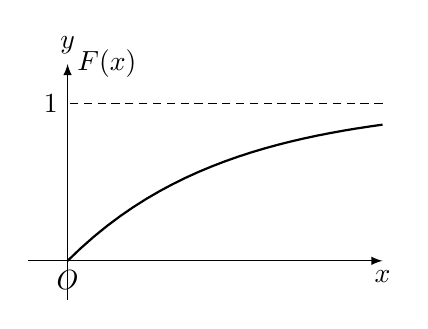
\begin{tikzpicture}[scale=2]
    \draw[-latex](-0.25,0) -- (2,0) node[below]{$x$};
    \draw[-latex](0,-0.25) -- (0,1.25) node[above]{$y$};
    \filldraw[black] (0,0) node[below]{$O$};
    \draw[black, densely dashed](2,1) -- (0,1) node[left]{$1$};
    \draw[black, thick, domain=0:2] plot (\x,{1-pow(e,-\x)});
    \filldraw[black] (0.25,1.25) node{$F(x)$};
\end{tikzpicture}

指数分布中$\lambda$代表失效率,往往用来代表一个事物毁坏的过程,如灯泡毁坏。

\textcolor{aqua}{\textbf{定理:}}无记忆性:若$X$服从指数分布,则$P\{X>s+t|X>s\}=P\{X>t\}$。

即在指数分布下事情发生的概率与前面所经过的时间无关,如果$T$是某一元件的寿命,已知元件使用了$t$小时,它总共使用至少$s+t$小时的条件概率,与从开始使用时算起它使用至少$s$小时的概率相等。

证明:$P\{X>s+t|X>s\}=\dfrac{P\{X>s+t\}}{P\{X>s\}}=\dfrac{1-P\{X\leqslant s+t\}}{1-P\{X\leqslant s\}}$

$=\dfrac{1-F(s+t)}{1-F(x)}=\dfrac{1-(1-e^{-\lambda(s+t)})}{1-(1-e^{-\lambda s})}=\dfrac{e^{-\lambda(s+t)}}{e^{-\lambda s}}=e^{-\lambda t}=1-(1-e^{-\lambda t})$

$=1-F(t)=1-P\{X\leqslant t\}=P\{X>t\}$。

\subsubsection{正态分布}

\textcolor{violet}{\textbf{定义:}}如果$X$的概率密度为$f(x)=\dfrac{1}{\sqrt{2\pi\delta}}e^{-\frac{1}{2}(\frac{x-\mu}{\delta})^2}$($-\infty<x<+\infty$,$-\infty<\mu<+\infty$,$\delta>0$),则称$X$服从参数为$(\mu,\delta^2)$的\textbf{正态分布},称$X$为\textbf{正态变量},记为$X\sim N(\mu,\delta^2)$。

$f(x)$的图形关于$x=\mu$对称,即$f(\mu-x)=f(\mu+x)$,并在$x=\mu$处有唯一最大值$f(\mu)=\dfrac{1}{\sqrt{2\pi}\delta}$。$\mu-\delta$和$\mu+\delta$为拐点。

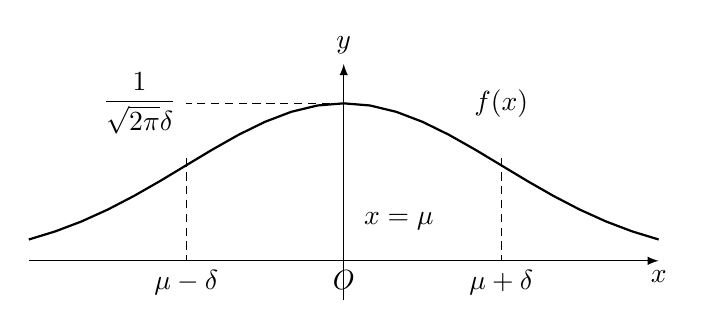
\begin{tikzpicture}[scale=2]
    \draw[-latex](-2,0) -- (2,0) node[below]{$x$};
    \draw[-latex](0,-0.25) -- (0,1.25) node[above]{$y$};
    \filldraw[black] (0,0) node[below]{$O$};
    \draw[black, thick, domain=-2:2] plot (\x,{pow(e,-\x*\x/2)});
    \draw[black, densely dashed](-1,0.65) -- (-1,0) node[below]{$\mu-\delta$};
    \draw[black, densely dashed](1,0.65) -- (1,0) node[below]{$\mu+\delta$};
    \draw[black, densely dashed](0,1) -- (-1,1) node[left]{$\dfrac{1}{\sqrt{2\pi}\delta}$};
    \filldraw[black] (0.35,0.25) node{$x=\mu$};
    \filldraw[black] (1,1) node{$f(x)$};
\end{tikzpicture}

当$\mu=0$,$\delta=1$时的正态分布$N(0,1)=\dfrac{1}{\sqrt{2\pi}}e^{-\frac{x^2}{2}}$为\textbf{标准正态分布},记为$\phi(x)$,分布函数为$\varPhi(x)=\displaystyle{\int_{-\infty}^x\dfrac{1}{\sqrt{2\pi}}e^{-\frac{t^2}{2}}\,\textrm{d}t}$。$\phi(x)$为偶函数,$\varPhi(0)=\dfrac{1}{2}$,$\varPhi(-x)=1-\varPhi(x)$。

若$X\sim N(0,1)$,$P\{X>\mu_\alpha\}=\alpha$,则称$\mu_\alpha$为标准正态分布的\textbf{上侧$\alpha$分位数/上$\alpha$分位点}。

若$X\sim N(\mu,\delta^2)$,则

\begin{itemize}
    \item $F(x)=P\{X\leqslant x\}=P\left\{\dfrac{X-\mu}{\delta}\leqslant\dfrac{x-\mu}{\delta}\right\}=\varPhi\left(\dfrac{x-\mu}{\delta}\right)$。(标准化)
    \item $F(\mu-x)+F(\mu+x)=1$。
    \item $P\{a<X<b\}=\varPhi\left(\dfrac{b-\mu}{\delta}\right)-\varPhi\left(\dfrac{a-\mu}{\delta}\right)$。(标准化得到)
    \item $aX+b\sim N(a\mu+b,a^2\theta^2)$($a\neq0$)。
\end{itemize}

\section{一维随机变量函数分布}

设$X$为随机变量,函数$y=g(x)$,则以随机变量$X$作为自变量的函数$Y=g(X)$也是随机变量,称为\textbf{随机变量$X$的函数}。

如$Y=aX^2+bX^+c$等等。

\subsection{离散型}

设$X$为离散型随机变量,其概率分布为$p_i=P\{X=x_i\}$($i=1,2,\cdots$),则$X$的函数$Y=g(X)$也是离散型随机变量,其概率分布为$P\{Y=g(x_i)\}=p_i$($i=1,2,\cdots$)。

即$Y\sim\left(\begin{array}{ccc}
    g(x_1) & g(x_2) & \cdots \\
    p_1 & p_2 & \cdots
\end{array}\right)$。

若有若干个$g(x_i)$相同,则合并为一项,并将对应概率相加作为$Y$取$g(x_i)$的概率。

离散型一维随机变量函数分布单独考的可能性很低。

\textbf{例题:}设$X$是仅可能取6个值的离散型随机变量,分布为:\medskip

\begin{tabular}{c|cccccc}
    \hline
    X & -2 & -1 & 0 & 1 & 2 & 3 \\ \hline
    P & 0.05 & 0.15 & 0.20 & 0.25 & 0.20 & 0.15 \\
    \hline
\end{tabular} \medskip

求$Y=2X+1$,$Z=X^2$的概率分布。

因为$Y=2X+1$是线性的,所以改变$X$变为$Y$,所对应的$P$不变:\medskip

\begin{tabular}{c|cccccc}
    \hline
    Y & -3 & -1 & 1 & 3 & 5 & 7 \\ \hline
    P & 0.05 & 0.15 & 0.20 & 0.25 & 0.20 & 0.15 \\
    \hline
\end{tabular} \medskip

对于$Z=X^2$是一个平方,导致$Z$的值有些是一样的,所以概率合在一起:\medskip

\begin{tabular}{c|cccc}
    \hline
    Z & 0 & 1 & 4 & 9 \\ \hline
    P & 0.20 & 0.40 & 0.25 & 0.15 \\
    \hline
\end{tabular}

\subsection{连续性}

设$X$为离散型随机变量,其分布函数、概率密度为$F_X(x)$与$f_X(x)$,随机变量$Y=g(X)$也是$X$的函数,则$Y$的分布函数或概率密度可用分布函数法得到$F_Y(y)=P\{Y\leqslant y\}=P\{g(X)\leqslant y\}=\int_{g(X)\leqslant y}f_X(x)\,\textrm{d}x$。

若$F_Y(y)$连续,且除有限个点外,$F_Y'(y)$存在且连续,$Y$的概率密度为$f_Y(y)=F_Y'(y)$。

首先已知$X$的概率密度函数为$f_X(x)$,分布函数为$F_X(x)$,已知$Y=g(X)$,即$Y$对$X$的映射关系。现在要求$Y$的概率规律,即要求$Y$的概率密度$f_Y(y)$与分布函数$F_Y(y)$。

先求分布函数$F_Y(y)=P\{Y\leqslant y\}=P\{g(X)\leqslant y\}$,然后用$y$来表示$X$,这是连续性随机变量函数分布的重点。

即$X$在以$y$表示的一个区间上,$X\in I_y$,所以解得$Y$分布函数$\int_{I_y}f_X(x)\,\textrm{d}x$。

\textbf{例题:}设随机变量$X$的概率密度为$f_X(x)=\left\{\begin{array}{ll}
    1+x, & -1\leqslant x<0 \\
    1-x, & 0\leqslant x\leqslant1 \\
    0, & \text{其他}
\end{array}\right.$,求随机变量$Y=X^2+1$的分布函数。

解:求随机变量$Y=X^2+1$的分布函数即求$F_Y(y)=P\{Y\leqslant y\}=P\{X^2+1\leqslant y\}$。即将$X^2+1$与$y$的概率关系解出,即求曲线$X^2+1$与直线$y$的关系。

根据$X$的概率密度函数,所以只有$x\in [-1,1]$才有正概率,其他区间概率为0,即不能取,将$Y$的取值范围划在$[-1,1]$中。

又由$f_X(x)$的关系知道$Y$的函数,是在$[-1,1]$的属于$[1,2]$的抛物线。

当$y<1$时,$Y=X^2+1>1$恒成立,所以$X^2+1\leqslant y$不可能发生,概率为0,所以$F_Y(y)=0$。

当$y>2$时,$Y=X^2+1$在$X\in[-1,1]$时$Y\in[1,2]$,所以$X^2+1\leqslant y$必然成立,所以所以$F_Y(y)=1$。

当$1<y<2$时,解出$X^2+1\leqslant y$为$X=\pm\sqrt{y-1}$,所以$F_Y(y)=P\{-\sqrt{y-1}\leqslant X\leqslant\sqrt{y-1}\}=\int_{-\sqrt{y-1}}^{\sqrt{y-1}}f(x)\,\textrm{d}x=\int_{-\sqrt{y-1}}^01+x\,\textrm{d}x+\int_0^{\sqrt{y-1}}1-x\,\textrm{d}x=2\sqrt{y-1}-y+1$。

\section{多维随机变量}

\subsection{概念}

多维随机变量\textcolor{violet}{\textbf{定义:}}如果$X_1,X_2,\cdots,X_n$是定义在同一个样本空间上的$n$个随机变量,则称$(X_1,X_2,\cdots,X_n)$为\textbf{$n$维随机变量}或\textbf{$n$维随机向量},$X_i$为第$i$个分量。

当$n=2$时,$(X,Y)$为\textbf{二维随机变量/二维随机向量}。

\subsection{联合分布函数}

\textcolor{violet}{\textbf{定义:}}对任意$n$个实数$x_1,x_2,\cdots,x_n$称为$n$元函数$F(x_1,x_2,\cdots,x_n)=P\{X_1\leqslant x_1,X_2\leqslant x_2,\cdots,X_n\leqslant x_n\}$为$n$为随机变量$(X_1,X_2,\cdots,X_n)$的\textbf{联合分布函数}。

当$n=2$时对任意的实数$xy$称二元函数$F(x,y)=P\{X\leqslant x,Y\leqslant y\}$为二维随机变量$(X,Y)$的\textbf{联合分布函数},简称\textbf{分布函数},记为$(X,Y)\sim F(x,y)$。

性质:

\begin{itemize}
    \item 单调性:$F(x,y)$是$xy$的单调不减函数。
    \item 右连续性:$F(x,y)$在右边连续。
    \item 有界性:当$x$或$y$趋向负无穷时值为0,当$x$和$y$趋向正无穷时值为1。
    \item 非负性:对任意$x_1<x_2$,$y_1<y_2$有$P\{x_1<X\leqslant x_2,y_1<Y\leqslant y_2\}=F(x_2,y_2)-F(x_2,y_1)-F(x_1,y_2)+F(x_1,y_1)\geqslant0$。(由定义画图可知)
\end{itemize}

\subsection{边缘分布函数}

\textcolor{violet}{\textbf{定义:}}设二维随机变量$(X,Y)$的联合分布函数为$F(x,y)$,随机变量$X,Y$的分布函数$F_X(x)$与$F_Y(y)$分别称$(X,Y)$关于$X$与关于$Y$的\textbf{边缘分布函数}。

$F_X(x)=P\{X\leqslant x\}=P\{X\leqslant x,Y<+\infty\}=\lim\limits_{y\to+\infty}P\{X\leqslant x,Y\leqslant y\}=\lim\limits_{y\to+\infty}F(x,y)=F(x,+\infty)$。同理$F_Y(y)=F(+\infty,y)$。

所以就可以通过联合分布函数推出边缘分布函数。

\section{二维离散型随机变量}

\textcolor{violet}{\textbf{定义:}}若二维随机变量$(X,Y)$只能取有限或可列对值$(x_1,y_1),(x_2,y_2),\cdots$则称$(X,Y)$为\textbf{二维离散型随机变量}。

\subsection{联合分布律}

\textcolor{violet}{\textbf{定义:}}$p_{ij}=P\{X=x_i,Y=y_j\}$,$i,j=1,2,\cdots$为$(X,Y)$的\textbf{分布律}或随机变量$X$和$Y$的\textbf{联合分布律},记为$(X,Y)\sim p_{ij}$。

数列$\{p_{ij}\}$,$i,j=1,2,\cdots$是某一二维离散型随机变量的概率分布的充要条件是$p_{ij}\geqslant0$,$\sum\limits_{i=1}^\infty\sum\limits_{j=1}^\infty p_{ij}=1$。

\textcolor{violet}{\textbf{定义:}}若$p_{ij}$,$i,j=1,2,\cdots$为$(X,Y)$的概率分布,则$(X,Y)$的\textbf{联合分布函数}为$F(x,y)=P\{X\leqslant x,Y\leqslant y\}=\sum\limits_{x_i\leqslant x}\sum\limits_{y_j\leqslant y}p_{ij}$。

联合分布函数是以$(x,y)$为定点的左下角平面上$(X,Y)$所有可能取值的概率的和。

设$G$是平面上某个区域,则$P\{(X,Y)\in G\}=\sum\limits_{(x_i,y_j)\in G}p_{ij}$。

\subsection{边缘分布律}

\textcolor{violet}{\textbf{定义:}}对于同一个$x$值的所有$y$取值的概率的和,就是该$x$值的\textbf{边缘分布律}。同理对于同一个$y$值的所有$x$取值的概率的和,就是该$y$值的\textbf{边缘分布律}。

即$p_{i\cdot}=P\{X=x_i\}=\sum\limits_{j=1}^\infty P\{X=x_i,Y=y_j\}=\sum\limits_{j=1}^\infty p_{ij}$($i=1,2,\cdots$)。

$p_{\cdot j}=P\{Y=y_i\}=\sum\limits_{i=1}^\infty P\{X=x_i,Y=y_j\}=\sum\limits_{i=1}^\infty p_{ij}$($j=1,2,\cdots$)。

\subsection{条件分布律}

条件分布律类比随机事件概率中的条件概率。

\textcolor{violet}{\textbf{定义:}}如果$(X,Y)\sim p_{ij}$($i,j=1,2,\cdots$),对固定的$j$,如果$p_{\cdot j}=P\{Y=y_j\}>0$,则称$P\{X=x_i|Y=y_j\}=\dfrac{P\{X=x_i,Y=y_j\}}{P\{Y=y_j\}}=\dfrac{p_{ij}}{p_{\cdot j}}$($i=1,2,\cdots$)为$X$在$Y=y_j$条件下的\textbf{条件分布}。

同理\textcolor{violet}{\textbf{定义:}}$Y$在$X=x_i$条件下的\textbf{条件分布}为$P\{Y=y_j|X=x_i\}=\dfrac{p_{ij}}{p_{i\cdot}}$($j=1,2,\cdots$)。

\section{二维连续型随机变量}

\textcolor{violet}{\textbf{定义:}}如果二维随机变量$(X,Y)$的联合分布函数$F(x,y)$可表示为$F(x,y)=\int_{-\infty}^x\int_{-\infty}^yf(u,v)\,\textrm{d}u\textrm{d}v$,($(x,y)\int R^2$),其中$f(x,y)$为非负可积函数,则称$(X,Y)$为\textbf{二维连续型随机变量},$f(x,y)$为$(X,Y)$的\textbf{概率密度},记为$(X,Y)\sim f(x,y)$。

二元函数$f(x,y)$是概率密度的充要条件$f(x,y)\geqslant0$,$\int_{-\infty}^{+\infty}\int_{-\infty}^{+\infty}f(x,y)\,\textrm{d}x\textrm{d}y$\\$=1$。

改变$f(x,y)$有限个点值(仍取非负值),$f(x,y)$仍是概率密度。

\subsection{联合概率密度}

\textcolor{violet}{\textbf{定义:}}设$(X,Y)$的联合分布函数为$F(x,y)$,概率密度为$f(x,y)$,则

\begin{itemize}
    \item $F(x,y)$为$(x,y)$的二元连续函数,且$F(x,y)=P\{X\leqslant x,Y\leqslant y\}=\int_{-\infty}^x\int_{-\infty}^xf(u,v)\,\textrm{d}u\textrm{d}v$。
    \item 设$G$为平面上某个区域,则$P\{(X,Y)\in G\}=\iint\limits_Gf(x,y)\,\textrm{d}x\textrm{d}y$。
    \item 若$f(x,y)$在点$(x,y)$处连续,则$\dfrac{\partial^2F(x,y)}{\partial x\partial y}=f(x,y)$。
    \item 若$F(x,y)$连续可导,则$(X,Y)$是连续型随机变量,则$\dfrac{\partial^2F(x,y)}{\partial x\partial y}$是其概率密度。
\end{itemize}

\subsection{边缘概率密度}

\textcolor{violet}{\textbf{定义:}}设$(X,Y)\sim f(x,y)$,则$X$的边缘分布函数为$F_X(x)=F(x,+\infty)=\int_{-\infty}^x\left[\int_{-\infty}^{+\infty}f(u,v)\,\textrm{d}v\right]\textrm{d}u$,所以$X$为连续型随机变量,其概率密度$f_X(x)=$\\$\int_{-\infty}^{+\infty}f(x,y)\,\textrm{d}y$,称$f_X(x)$为$(X,Y)$关于$X$的\textbf{边缘概率密度}。同理$Y$也为连续型随机变量,其概率密度为$f_Y(y)=\int_{-\infty}^{+\infty}f(x,y)\,\textrm{d}x$。

\subsection{条件概率密度}

\textcolor{violet}{\textbf{定义:}}设$(X,Y)\sim f(x,y)$,边缘概率密度$f_X(x)>0$,则称$f_{Y|X}(y|x)=\dfrac{f(x,y)}{f_X(x)}$为$Y$在$X=x$条件下的\textbf{条件概率密度}。同理$X$在$Y=y$条件下的条件概率密度为$f_{X|Y}(x|y)=\dfrac{f(x,y)}{f_Y(y)}$。

若$f_X(x)>0$,$f_Y(y)>0$,则有概率密度乘法公式$f(x,y)=f_X(x)f_{Y|X}(y|x)=f_Y(y)f_{X|Y}(x|y)$。

\textcolor{violet}{\textbf{定义:}}$Y$在$X=x$条件下的\textbf{条件分布函数}为$F_{Y|X}(y|x)=\int_{-\infty}^yf_{Y|X}(y|x)\,\textrm{d}y=\int_{-\infty}^y\dfrac{f(x,y)}{f_X(x)}\textrm{d}y$,同理$X$在$Y=y$条件下的条件分布函数为$F_{X|Y}(x|y)$

\subsection{二维均匀分布}

\subsection{二维正态分布}

\section{随机变量独立性}

\subsection{概念}

\subsection{充要条件}

\subsection{性质}

\section{二维随机变量函数分布}

\subsection{离散型}

\subsection{连续型}

\subsection{混合型}

\end{document}
